\documentclass[11pt]{article}

% ---------------------------------------------------------------------------
%  Preamble (pdflatex-safe)
% ---------------------------------------------------------------------------
\usepackage[a4paper,margin=1.8cm]{geometry}
\usepackage{amsmath,amssymb}
\usepackage{tikz}
\usepackage{tikz-cd}
\usetikzlibrary{arrows.meta,positioning,calc,fit,backgrounds,
  shapes.geometric,decorations.pathreplacing,decorations.markings}
\usepackage[most]{tcolorbox}
\usepackage{listings}
\usepackage{parskip}
\usepackage{xcolor}

\definecolor{ink}{RGB}{40,40,40}
\definecolor{soft}{RGB}{245,245,248}
% the four "pattern" colours
\definecolor{cAct}{RGB}{30,90,160}    % monoid action / delooping
\definecolor{cNNO}{RGB}{30,140,80}    % NNO / recursor
\definecolor{cRing}{RGB}{200,120,0}   % endomorphism ring / augmentation
\definecolor{cTr}{RGB}{150,60,160}    % categorical trace
\definecolor{cInp}{RGB}{190,50,60}    % genuine arithmetic input
\definecolor{res}{RGB}{190,50,60}

% ----- Lean listing style (unicode via listings literate) -----
\definecolor{leanbg}{RGB}{248,248,252}
\definecolor{leankw}{RGB}{140,20,140}
\definecolor{leancm}{RGB}{110,120,130}
\lstdefinestyle{lean}{
  basicstyle=\ttfamily\footnotesize,
  backgroundcolor=\color{leanbg},
  frame=single, framesep=4pt, rulecolor=\color{gray!40},
  breaklines=true, columns=fullflexible, keepspaces=true,
  keywordstyle=\color{leankw}\bfseries,
  commentstyle=\color{leancm}\itshape,
  morecomment=[l]{--},
  morekeywords={theorem,lemma,def,by,namespace,end,variable,open,rw,exact,
    have,intro,induction,with,fun,Prop,Field,Fintype,CharP,set,apply,refine,
    rcases,cases,unfold,simp,ring,ring_nf,grind,linear_combination,omit,in,
    positivity,conv_lhs,show,from,where,noncomputable,Type,MonoidHom},
  literate=
    {∑}{{$\sum$}}1 {∈}{{$\in$}}1 {ℕ}{{$\mathbb{N}$}}1 {→}{{$\to$}}1
    {≠}{{$\neq$}}1 {∨}{{$\vee$}}1 {∧}{{$\wedge$}}1 {∀}{{$\forall$}}1
    {·}{{$\cdot$}}1 {ℓ}{{$\ell$}}1 {≡}{{$\equiv$}}1 {𝔽}{{$\mathbb{F}$}}1
    {⟹}{{$\Rightarrow$}}1 {⟨}{{$\langle$}}1 {⟩}{{$\rangle$}}1
    {≤}{{$\le$}}1 {↦}{{$\mapsto$}}1 {←}{{$\leftarrow$}}1 {×}{{$\times$}}1
    {σ}{{$\sigma$}}1 {φ}{{$\varphi$}}1 {Φ}{{$\Phi$}}1 {τ}{{$\tau$}}1
    {θ}{{$\theta$}}1 {μ}{{$\mu$}}1 {ν}{{$\nu$}}1 {ρ}{{$\rho$}}1
    {γ}{{$\gamma$}}1 {β}{{$\beta$}}1 {α}{{$\alpha$}}1 {κ}{{$\kappa$}}1
    {ε}{{$\varepsilon$}}1 {∘}{{$\circ$}}1 {⥤}{{$\rightsquigarrow$}}1
    {²}{{\textsuperscript{2}}}1 {ⁿ}{{\textsuperscript{n}}}1
    {ⁱ}{{\textsuperscript{i}}}1 {ʲ}{{\textsuperscript{j}}}1
    {≃}{{$\simeq$}}1 {ₙ}{{$_n$}}1
}
\lstset{style=lean}
\DeclareUnicodeCharacter{2080}{\ensuremath{_0}}
\DeclareUnicodeCharacter{2081}{\ensuremath{_1}}

\newtcolorbox{note}[1][]{colback=soft,colframe=ink,boxrule=0.4pt,
  arc=2pt,left=6pt,right=6pt,top=4pt,bottom=4pt,#1}

\tikzset{
  obj/.style={draw=ink,rounded corners=3pt,fill=soft,inner sep=5pt,
    font=\small,align=center},
  ar/.style={-{Stealth[length=2.2mm]},shorten >=1pt,shorten <=1pt},
  tag/.style={font=\footnotesize\itshape,inner sep=1pt},
}
\newcommand{\lc}[1]{\texttt{\small #1}}
\newcommand{\Tr}{\operatorname{Tr}}
\newcommand{\Nn}{\mathbb{N}}
\newcommand{\Fq}{\mathbb{F}_{2^{n}}}
\newcommand{\End}{\operatorname{End}}
\newcommand{\B}{\mathrm{B}}

\title{\bfseries The Categorical Patterns of the\\
  Dobbertin $(1)\!\Rightarrow\!(2)$ Formalisation\\[4pt]
  \large A TikZ field-guide to \lc{DobbertinLego/Categorical.lean} and its
  golfed mirror \lc{G/Cat.lean}}
\author{}
\date{}

\begin{document}
\maketitle

\begin{abstract}
The Lean formalisation of the opening step $(1)\Rightarrow(2)$ of Dobbertin's
Theorem~1 is assembled from a handful of components --- \emph{Frobenius}, the
\emph{loop/trace}, the \emph{endomorphism}, the \emph{telescope}, and the
characteristic-$2$ inputs.  This note traces each component back to its most
abstract categorical home, and pairs the picture with the exact Lean
declarations that realise it (module \lc{DobbertinLego.Categorical}, golfed
mirror \lc{G.Cat}).  The upshot is a clean four-pattern reading: Frobenius is a
\emph{monoid action} (a functor on the delooping $\B\Nn$); the loop is the
\emph{norm element} generated by the \emph{natural-number-object recursor}; the
telescope is multiplication by the \emph{augmentation} $\varphi-1$ in the
endomorphism \emph{ring} (the geometric series); and the absolute trace is the
\emph{categorical (evaluation/coevaluation) trace}, equal to Mathlib's
\lc{Algebra.trace}.  Two facts --- additivity of Frobenius (char~$2$) and its
finite order (Fermat) --- are the irreducible arithmetic inputs where the
abstract scaffold meets the finite field.
\end{abstract}

% ===========================================================================
\section{The dictionary}

Every row is a theorem or definition in \lc{DobbertinLego.Categorical}
(golfed name in \lc{G.Cat} in the last column).

\begin{center}\small
\renewcommand{\arraystretch}{1.35}
\begin{tabular}{@{}p{3.1cm}p{6.4cm}p{3.0cm}p{2.0cm}@{}}
\hline
\textbf{component} & \textbf{categorical foundation} & \textbf{Lean (Categorical)} & \textbf{golfed}\\
\hline
\textcolor{cAct}{Frobenius $\varphi$ (shift)} &
  monoid action $\mathrm{Mult}\,\Nn \to \End$; a functor $\B\Nn\rightsquigarrow\mathbf{Type}$ &
  \lc{frobAction}, \lc{frobFunctor} & \lc{$\alpha$}, \lc{$\gamma$}\\
\textcolor{cNNO}{loop / trace $\sigma$} &
  norm element $\sum\varphi^{i}$, built by the \textbf{NNO} recursor on $\Nn$ &
  \lc{iterSum}, \lc{iterSum\_rec\_unique} & \lc{$\sigma$}, \lc{$\rho$}\\
\textcolor{cRing}{telescope} &
  multiply by augmentation $\varphi-1$ in the ring $\End A$ (geometric series) &
  \lc{augmentation\_mul\_normElt} & \lc{$\mu$}\\
\textcolor{cInp}{finite order / bit} &
  $\varphi^{n}=1$ (cyclic Galois group) forces $\sigma$ into the fixed subobject &
  \lc{iterSum\_fixed\_of\_orderly} & \lc{$\theta$}\\
\textcolor{cTr}{absolute trace $\Tr$} &
  categorical trace (eval/coeval loop) $=$ \lc{Algebra.trace} $\mathbb{F}_2\,F$ &
  \lc{trace\_eq\_algebraMap\_trace} & \lc{$\kappa$}\\
\textcolor{cInp}{characteristic $2$} &
  the \emph{input} making $\varphi$ an endomorphism of the \emph{additive} group &
  \lc{frob\_add} & \lc{$\varphi$a}\\
\hline
\end{tabular}
\end{center}

\begin{note}
\textbf{Reading.} The four coloured patterns (\textcolor{cAct}{action},
\textcolor{cNNO}{recursor}, \textcolor{cRing}{augmentation},
\textcolor{cTr}{trace}) are \emph{formal}: they hold for any endomorphism of any
abelian group / any dualizable object. The two \textcolor{cInp}{red} rows are the
only genuine finite-field inputs.
\end{note}

% ===========================================================================
\section{Pattern 1 --- Frobenius is the shift: a monoid action / delooping}

Additivity (\lc{frob\_add}) makes each iterate $\varphi^{r}$ an endomorphism of
the additive group $F$; composition (\lc{frob\_comp}) makes
$r\mapsto\varphi^{r}$ a \emph{monoid homomorphism} out of the free monoid on one
generator, $\mathrm{Mult}\,\Nn$. Equivalently it is a \emph{functor} out of the
one-object category $\B\Nn=\lc{SingleObj (Multiplicative }\Nn\lc{)}$, i.e.\ an
action of $\Nn$ on $F$.

\begin{center}
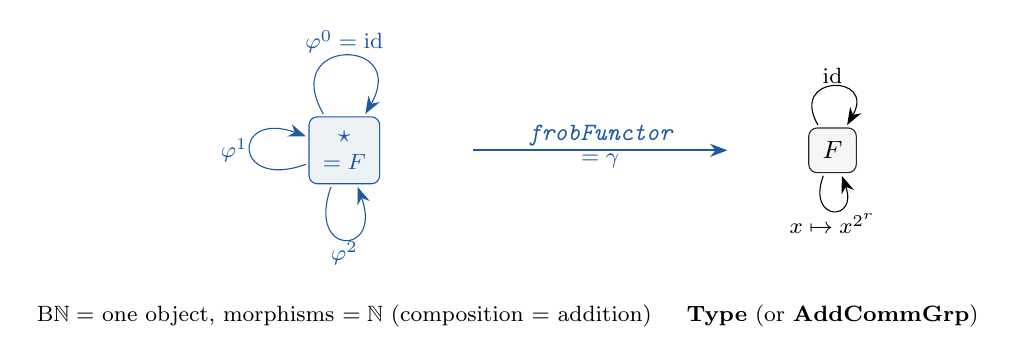
\begin{tikzpicture}[scale=1]
  % delooping BN : single object with self-loops
  \node[obj,cAct,draw=cAct,fill=cAct!8] (star) at (0,0) {$\star$\\[-1pt]\footnotesize $=F$};
  \draw[ar,cAct] (star) to[out=120,in=60,looseness=6] node[tag,above]{$\varphi^{0}=\mathrm{id}$} (star);
  \draw[ar,cAct] (star) to[out=200,in=160,looseness=8] node[tag,left]{$\varphi^{1}$} (star);
  \draw[ar,cAct] (star) to[out=250,in=290,looseness=8] node[tag,below]{$\varphi^{2}$} (star);
  \node at (0,-2.1) {\footnotesize $\B\Nn=$ one object, morphisms $=\Nn$ (composition $=$ addition)};

  % functor to Type
  \node[obj] (F) at (6.2,0) {$F$};
  \draw[ar] (F) to[out=120,in=60,looseness=6] node[tag,above]{$\mathrm{id}$} (F);
  \draw[ar] (F) to[out=250,in=290,looseness=8] node[tag,below]{$x\mapsto x^{2^{r}}$} (F);
  \draw[ar,cAct,thick] (1.6,0) -- node[tag,above]{\lc{frobFunctor}} node[tag,below]{$=\gamma$} (4.9,0);
  \node at (6.2,-2.1) {\footnotesize $\mathbf{Type}$ (or $\mathbf{AddCommGrp}$)};
\end{tikzpicture}
\end{center}

\begin{lstlisting}
noncomputable def frobAction : Multiplicative ℕ →* AddMonoid.End F where
  toFun r := frobEndo (Multiplicative.toAdd r)     -- r ↦ φ^r
  map_one' := ...   -- φ^0 = id
  map_mul' := ...   -- φ^(a+b) = φ^a ∘ φ^b

noncomputable def frobFunctor : SingleObj (Multiplicative ℕ) ⥤ Type _ :=
  SingleObj.functor frobTypeHom          -- BN ⥤ Type : the ℕ-action as a functor
\end{lstlisting}

\begin{note}
A functor out of \lc{SingleObj M} is \emph{exactly} an action of the monoid $M$
(Mathlib's \lc{SingleObj.functor} takes a monoid hom $M\to\End X$). Finiteness
of the field makes the action \emph{factor through the cyclic quotient}
$\mathrm{Mult}(\Nn/n\Nn)$ --- the Galois group $\mathrm{Gal}(\Fq/\mathbb{F}_2)$
generated by Frobenius --- because $\varphi^{n}=1$ (Pattern~1$'$, \lc{frobEndo\_pow\_card}).
\end{note}

% ===========================================================================
\section{Pattern 2 --- the loop is the norm element, built by the NNO recursor}

The loop $\sigma\,\varphi\,\ell = \sum_{i<\ell}\varphi^{i}$ is generated by the
inductive pattern: it is the \emph{unique} map $\Nn\to A$ with $g\,0=0$ and
$g(\ell+1)=g\,\ell+\varphi^{\ell}x$. This is precisely the recursor of a
natural-number object (the initial algebra of $X\mapsto \mathbf 1+X$).

\begin{center}
\begin{tikzcd}[column sep=large,row sep=large]
\mathbf 1 \arrow[r,"0"] \arrow[dr,swap,"z=0"] &
  \Nn \arrow[r,"{\mathrm{succ}}"] \arrow[d,dashed,"{g}"] &
  \Nn \arrow[d,dashed,"{g}"]\\
& A \arrow[r,swap,"{a\,\mapsto\, a+\varphi^{\ell}x}"] & A
\end{tikzcd}
\end{center}

The unique fill-in $g$ is $\ell\mapsto\sigma\,\varphi\,\ell\,x$; \lc{iterSum\_rec\_unique}
records exactly this universal property (Mathlib has no \lc{NNO} class, so the
recursor is stated directly).

\begin{lstlisting}
theorem iterSum_rec_unique (φ : AddMonoid.End A) (x : A) (g : ℕ → A)
    (h0 : g 0 = 0) (hs : ∀ len, g (len + 1) = g len + (φ ^ len) x) :
    ∀ len, g len = iterSum φ len x
\end{lstlisting}

% ===========================================================================
\section{Pattern 3 --- the telescope is the augmentation in the endomorphism ring}

Both Artin--Schreier telescopes the paper uses are one ring identity. In the
(noncommutative) endomorphism \emph{ring} $\End A$, the norm element
$N=\sum_{i<\ell}\varphi^{i}$ times the \emph{augmentation} $\varphi-1$ is the
geometric series $\varphi^{\ell}-1$:
\[
  (\varphi-1)\cdot N \;=\; \varphi^{\ell}-1
  \qquad(\text{Mathlib's }\lc{mul\_geom\_sum}).
\]
Applying this endomorphism to $x$ gives the pointwise telescope
$\varphi(\sigma x)-\sigma x=\varphi^{\ell}x-x$; over $\mathbb{F}_2$ the
subtraction becomes addition, giving the paper's ``add the $2^{k}$-th power to
itself''.

\begin{center}
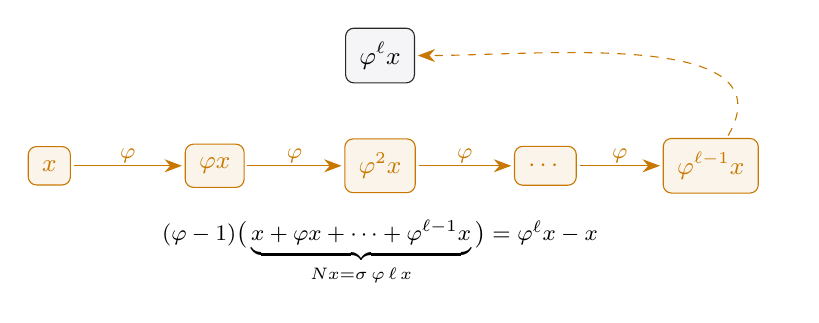
\begin{tikzpicture}[scale=1,every node/.style={font=\footnotesize}]
  \foreach \i/\lab in {0/x,1/{\varphi x},2/{\varphi^{2}x},3/{\cdots},4/{\varphi^{\ell-1}x}} {
    \node[obj,cRing,draw=cRing,fill=cRing!8] (n\i) at (\i*2.1,0) {$\lab$};
  }
  \foreach \i in {0,1,2,3} {
    \pgfmathtruncatemacro\j{\i+1}
    \draw[ar,cRing] (n\i) -- node[tag,above]{$\varphi$} (n\j);
  }
  \node[obj] (top) at (4.2,1.4) {$\varphi^{\ell}x$};
  \draw[ar,dashed,cRing] (n4) to[out=60,in=0] (top);
  \node at (4.2,-1.1) {$(\varphi-1)\big(\underbrace{x+\varphi x+\cdots+\varphi^{\ell-1}x}_{N x=\sigma\,\varphi\,\ell\,x}\big)=\varphi^{\ell}x-x$};
\end{tikzpicture}
\end{center}

\begin{lstlisting}
def normElt (φ : AddMonoid.End A) (len : ℕ) : AddMonoid.End A := ∑ i ∈ range len, φ ^ i
theorem augmentation_mul_normElt (φ : AddMonoid.End A) (len : ℕ) :
    (φ - 1) * normElt φ len = φ ^ len - 1 := mul_geom_sum φ len
\end{lstlisting}

\begin{note}
\textbf{Finite-order corollary (the ``bit'').} When $\varphi^{n}=1$ the right-hand
side is $0$, so $N$ maps $A$ into the fixed subgroup $\ker(\varphi-1)=A^{\varphi}$.
Over $\Fq$ this is $\mathbb{F}_2=\{0,1\}$, so $\Tr(x)$ is a bit
(\lc{iterSum\_fixed\_of\_orderly} $\to$ \lc{trace\_isBit}; golfed \lc{$\theta$}$\to$\lc{Tb}).
\end{note}

% ===========================================================================
\section{Pattern 4 --- the absolute trace is the categorical trace}

The absolute trace $\Tr(x)=\sum_{i<n}x^{2^{i}}$ is not an ad-hoc sum: it is the
\emph{categorical trace} of the multiplication endomorphism $m_x$ on the
dualizable object $F$ (a finite-dimensional $\mathbb{F}_2$-vector space) --- the
one ``open a loop with coevaluation, insert $m_x$, close it with evaluation''
move. Mathlib packages that value as \lc{Algebra.trace}, and computes it over the
prime field as the Frobenius sum, which is exactly the loop.

\begin{center}
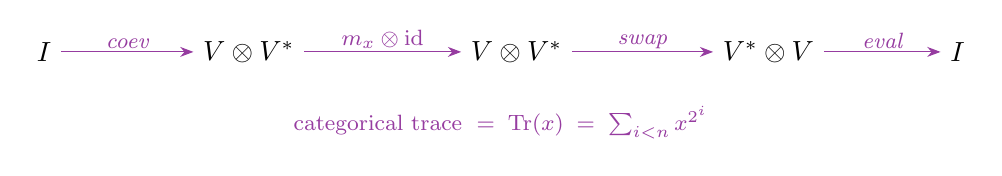
\begin{tikzpicture}[scale=1,>=Stealth]
  \node (I1) at (0,0) {$I$};
  \node (VV) at (2.6,0) {$V\otimes V^{*}$};
  \node (VV2) at (6.0,0) {$V\otimes V^{*}$};
  \node (VVs) at (9.2,0) {$V^{*}\otimes V$};
  \node (I2) at (11.6,0) {$I$};
  \draw[->,cTr] (I1) -- node[tag,above]{coev} (VV);
  \draw[->,cTr] (VV) -- node[tag,above]{$m_x\otimes\mathrm{id}$} (VV2);
  \draw[->,cTr] (VV2) -- node[tag,above]{swap} (VVs);
  \draw[->,cTr] (VVs) -- node[tag,above]{eval} (I2);
  \node[cTr] at (5.8,-0.9) {\footnotesize categorical trace $\;=\;\Tr(x)\;=\;\sum_{i<n}x^{2^{i}}$};
\end{tikzpicture}
\end{center}

\begin{lstlisting}
theorem trace_eq_algebraMap_trace (x : F) :
    letI := ZMod.algebra F 2
    trace (Module.finrank (ZMod 2) F) x
      = algebraMap (ZMod 2) F (Algebra.trace (ZMod 2) F x)
\end{lstlisting}

\begin{note}
The identification is genuine, not aspirational: at full length
$n=[F:\mathbb{F}_2]$ the paper's \lc{trace} equals Mathlib's \lc{Algebra.trace}
pushed back along \lc{algebraMap}, via \lc{FiniteField.algebraMap\_trace\_eq\_sum\_pow}.
\emph{Additivity} of $\Tr$ is then just monoidality/linearity --- no ad-hoc
computation.
\end{note}

% ===========================================================================
\section{Formal vs.\ arithmetic: where the field enters}

\begin{center}\small
\renewcommand{\arraystretch}{1.3}
\begin{tabular}{@{}p{7.2cm}p{7.4cm}@{}}
\hline
\textbf{Formal (any endomorphism / any abelian group)} &
\textbf{Genuine finite-field input} \\
\hline
telescope $(\varphi-1)N=\varphi^{\ell}-1$ (\lc{$\mu$}) &
  \textcolor{cInp}{char $2$: $\varphi$ additive} (\lc{$\varphi$a}, \lc{frob\_add})\\
$N$ lands in fixed points when $\varphi^{n}=1$ (\lc{$\theta$}) &
  \textcolor{cInp}{Fermat: $\varphi^{n}=1$} (\lc{$\Phi$F}, \lc{frobEndo\_pow\_card})\\
$\sigma$ as NNO recursor (\lc{$\rho$}) &
  \textcolor{cInp}{$A^{\varphi}=\mathbb{F}_2$ is a two-element set (the bit)}\\
Frobenius action / delooping (\lc{$\alpha$},\lc{$\gamma$}) &
  periodicity mod $n$ (\lc{$\varphi$p}) from $x^{|F|}=x$\\
\hline
\end{tabular}
\end{center}

Category theory supplies the \emph{shape} (a contraction/loop on a dualizable
object with a distinguished endomorphism); the two red facts supply the
\emph{content} at the point of specialization to $\Fq$.

% ===========================================================================
\section{The whole picture}

Each abstract pattern (left) specializes to a concrete brick over $\Fq$ (middle)
and feeds the headline $(1)\Rightarrow(2)$ (right). Golfed names in brackets.

\begin{center}
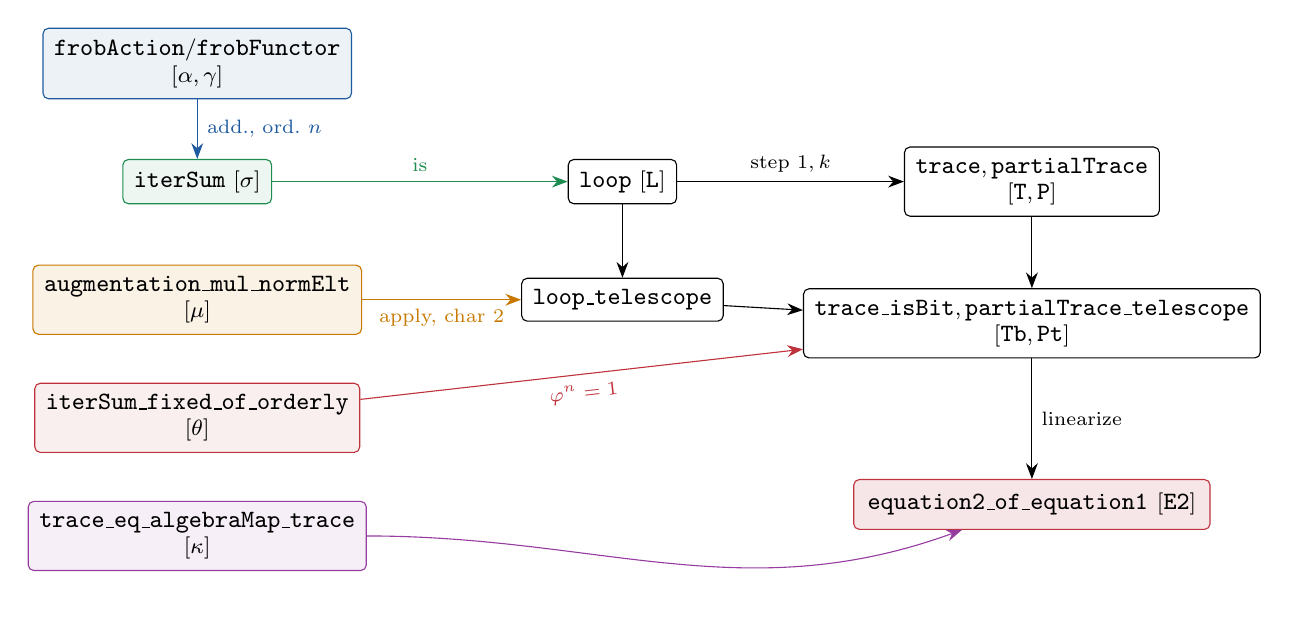
\begin{tikzpicture}[
  every node/.style={font=\footnotesize},
  box/.style={draw,rounded corners=2pt,align=center,inner sep=4pt},
   hd/.style ={draw,rounded corners=2pt,align=center,inner sep=5pt,
               fill=res!12,draw=res,font=\footnotesize\bfseries},
  fl/.style={-{Stealth[length=2mm]}}]
  % left column : abstract patterns
  \node[box,draw=cAct,fill=cAct!8]  (act) at (0,3.0)  {\lc{frobAction}/\lc{frobFunctor}\\ $[\alpha,\gamma]$};
  \node[box,draw=cNNO,fill=cNNO!8]  (nno) at (0,1.5)  {\lc{iterSum} $[\sigma]$};
  \node[box,draw=cRing,fill=cRing!10](rng) at (0,0.0)  {\lc{augmentation\_mul\_normElt}\\ $[\mu]$};
  \node[box,draw=cInp,fill=cInp!8]  (fix) at (0,-1.5) {\lc{iterSum\_fixed\_of\_orderly}\\ $[\theta]$};
  \node[box,draw=cTr,fill=cTr!8]    (tr)  at (0,-3.0) {\lc{trace\_eq\_algebraMap\_trace}\\ $[\kappa]$};
  % middle column : concrete bricks
  \node[box] (loop) at (5.4,1.5)  {\lc{loop} $[\lc{L}]$};
  \node[box] (tel)  at (5.4,0.0)  {\lc{loop\_telescope}};
  % right column : paper facts and headline
  \node[box] (tp)   at (10.6,1.5) {\lc{trace},\,\lc{partialTrace}\\ $[\lc{T},\lc{P}]$};
  \node[box] (bit)  at (10.6,-0.3){\lc{trace\_isBit},\,\lc{partialTrace\_telescope}\\ $[\lc{Tb},\lc{Pt}]$};
  \node[hd]  (head) at (10.6,-2.6){\lc{equation2\_of\_equation1} $[\lc{E2}]$};
  % edges
  \draw[fl,cAct] (act) -- node[right]{\scriptsize add., ord.\ $n$} (nno);
  \draw[fl,cNNO] (nno) -- node[above]{\scriptsize is} (loop);
  \draw[fl,cRing](rng) -- node[below]{\scriptsize apply, char $2$} (tel);
  \draw[fl] (loop) -- node[above,sloped]{\scriptsize step $1,k$} (tp);
  \draw[fl] (tel)  -- (bit);
  \draw[fl] (loop) -- (tel);
  \draw[fl,cInp] (fix) -- node[below,sloped]{\scriptsize $\varphi^{n}=1$} (bit);
  \draw[fl] (tp)  -- (bit);
  \draw[fl] (bit) -- node[right]{\scriptsize linearize} (head);
  \draw[fl,cTr] (tr) to[out=0,in=200] (head);
\end{tikzpicture}
\end{center}

\begin{note}
\textbf{Soundness.} \lc{DobbertinLego.Categorical} and the golfed \lc{G} library
build \lc{sorry}-free; every headline (\lc{trace\_eq\_algebraMap\_trace},
\lc{augmentation\_mul\_normElt}, \lc{equation2\_of\_equation1} / \lc{E2}, $\dots$)
depends only on \lc{propext}, \lc{Classical.choice}, \lc{Quot.sound}. The
categorical layer \emph{organises} the proof; the arithmetic is discharged by the
two red inputs.
\end{note}

\end{document}
